\chapter{Semantiche basate su Labelling} \label{ch:Semantiche basate su Labelling}
\section{Semantiche basate su Labelling}
Il Labeling è una funzione che assegna delle etichette rappresentate come colori ad ogni argomento. Le etichette sono di tre tipi:
\begin{enumerate}
    \item \textbf{Verdi:} Corrispondono ad argomenti IN, cioè sono ”dentro” l’insieme di argomenti accettati.
    \item \textbf{Rosse:} Corrispondono ad argomenti OUT, cioè sono ”fuori” dall’insieme di argomenti accettati.
    \item \textbf{Gialle:} ”Undecided” e sono fuori dagli insiemi direttamente accettati(verdi) ma non sono direttamente Rejected (rossi), ovvero non ho una motivazione esplicita per non accettare quel nodo, quindi sono una via di mezzo.
\end{enumerate}
Qualsiasi assegnamento di colori è un labeling (posso colorare tutti i nodi di verde e apposto), però chiaramente non rispetterà le semantiche che adesso introdurremo. Le semantiche basate su labeling corrispondono esattamente alle semantiche basate su estenzioni, ed infatti possiamo calcolare le stesse
cose.
\newpage
\subsection{Conflict-Free Labeling Based}
Per ogni argomento $a \in A$ si ha che:
\begin{itemize}
    \item $a$ è \textbf{IN} se non ha altri attaccanti IN.
    \item $a$ è \textbf{OUT} se è attaccato da almeno un argomento IN.
\end{itemize}
\begin{figure}[htp]
	\centering
    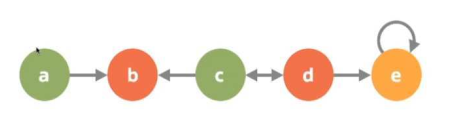
\includegraphics[width=12cm, keepaspectratio]{img/Cap7/CF.png}
    \caption{Esempio di Conflict-Free Labeling.}
\end{figure}
\begin{itemize}
    \item $a$ è verde perchè non ha nessun altro argomento verde che lo attacca.
    \item $c$ è verde per lo stesso motivo
    \item $b$ e $d$ sono rossi perchè c’è almeno un argomento verde che li attacca.
    \item $e$ è attaccato da un argomento rosso, ma le regole non specificano il colore in questo caso, quindi l’argomento resta fuori sia dalla colorazione IN che OUT. Per esprimere questa incertezza utilizzo la label gialla.
\end{itemize}
\textbf{Domanda: } Questo labeling sotto è conflict free? (cioè soddisfa le regole scritte sopra?)
\begin{figure}[htp]
	\centering
    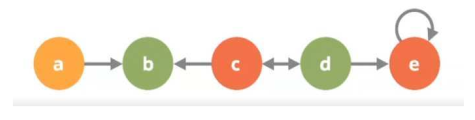
\includegraphics[width=12cm, keepaspectratio]{img/Cap7/CF2.png}
    \caption{Conflict free label}
\end{figure}
\begin{center}
    \textbf{Si, nessuna regola viene violata.}
\end{center}
\newpage
\textbf{Domanda: } Questo labeling sotto è conflict free?
\begin{figure}[htp]
	\centering
    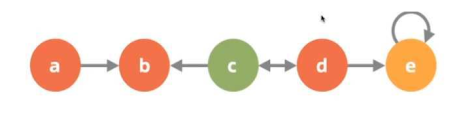
\includegraphics[width=12cm, keepaspectratio]{img/Cap7/CF3.png}
    \caption{No conflict free label}
\end{figure}
\begin{center}
    \textbf{No! perchè a è rosso ma non ha un argomento verde che lo attacca.}
\end{center}
\newpage
\subsection{Labeling Admissible}
Per ogni argomento $a \in A$ si ha che:
\begin{itemize}
    \item $a$ è \textbf{IN} se tutti i suoi attaccanti sono OUT.
    \item $a$ è \textbf{OUT} se è attaccato da almeno un argomento IN. In questo caso c’è la nozione di Difesa, ovvero che un argomento è accettato (è IN) solamente se tutti i suoi attaccanti sono sconfitti (OUT)
\end{itemize}
In questo caso c’è la nozione di Difesa, ovvero che un argomento è accettato (è IN) solamente se \textbf{tutti} i suoi attaccanti sono sconfitti (OUT)
\begin{figure}[htp]
	\centering
    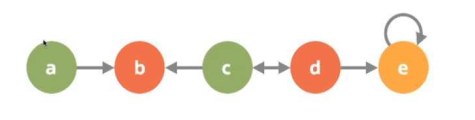
\includegraphics[width=12cm, keepaspectratio]{img/Cap7/LA.png}
    \caption{Esempio Labeling Admissible}
\end{figure}
\\Questo labeling è admissible, ad esempio c è accettato perchè d che lo attacca è sconfitto, cioè OUT.
\begin{figure}[htp]
	\centering
    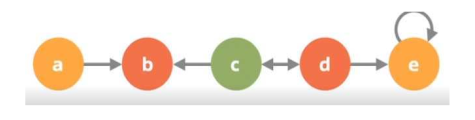
\includegraphics[width=12cm, keepaspectratio]{img/Cap7/LA2.png}
    \caption{Esempio2 Labeling Admissible}
\end{figure}
Questo esempio è comunque admissible, perchè non ho obblighi sull’argomento a, posso etichettarlo di Verde e la regola sarebbe soddisfatta, ma non avendo attaccanti posso etichettarlo sia giallo che verde e non violo nessuna regola.
\begin{center}
    \textbf{Differenza}
\end{center}
La differenza tra Admissible e Complete è che A in complete deve essere per forza verde mentre qui può essere anche giallo.
\newpage
\subsection{Labeling Complete}
Per ogni argomento $a \in A$ si ha che:
\begin{itemize}
    \item  $a$ è \textbf{IN} $se e solo se$ tutti i suoi attaccanti sono etichettati come OUT o quell’argomento non ha attaccanti.
    \item $a$ è \textbf{OUT} $se e solo se$ è attaccato da almeno un argomento IN.
\end{itemize}
\textbf{Domanda: } Questo labeling è complete?
\begin{figure}[htp]
	\centering
    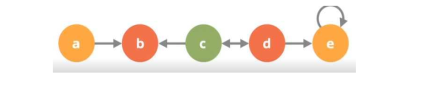
\includegraphics[width=12cm, keepaspectratio]{img/Cap7/LC.png}
    \caption{Esempio Labeling NON COMPLETE}
\end{figure}
\\No, perchè l’argomento a è etichettato di giallo, ma la prima regola mi dice che un argomento è etichettato di verde quando tutti i suoi attaccanti sono etichettati di rosso, ma ho un se e solo se, devo leggerlo anche dalla parte opposta, ovvero:

\vspace{0.3cm}

É IN se ha tutti attaccanti etichettati OUT, ma dato che a non ha attaccanti deve per forza essere verde, cosi come d.

\vspace{0.3cm}

\textbf{La differenza} con l’admissible è proprio quel ”se e solo se”. L’admissible ci permette di ignorare degli elementi che potrebbero essere accettati (infatti posso sia etichettarlo verde o giallo a prima), ma questo non accade nella complete, cioè se tutti gli argomenti che mi attaccano sono out (e questo
accade anche quando nessun argomento mi attacca) allora devo essere per forza verde. 
\\
Il labeling complete dell’esempio sarebbe:
\begin{figure}[htp]
	\centering
    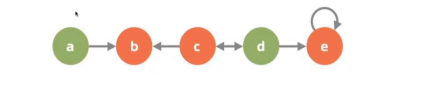
\includegraphics[width=12cm, keepaspectratio]{img/Cap7/LC2.png}
    \caption{Esempio Labeling COMPLETE}
\end{figure}
\newpage
\subsection{Labeling Grounded (Minimale)}
Il labeling deve essere:
\begin{itemize}
    \item \textbf{Completo}ù
    \item L’insieme degli argomenti \textbf{IN} deve essere \textbf{Minimale} tra tutte le labeling complete.
\end{itemize}
\subsection{Labeling Prefered (Massimale)}
\begin{itemize}
    \item \textbf{Completo}
    \item L’insieme degli argomenti \textbf{IN} deve essere \textbf{Massimale} tra tutte le labeling complete.
\end{itemize}
\begin{figure}[htp]
	\centering
    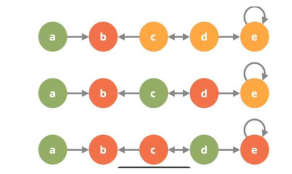
\includegraphics[width=12cm, keepaspectratio]{img/Cap7/GR.png}
\end{figure}
Di queste:
\begin{enumerate}
    \item \textbf{Grounded} perchè solo l’argomento $a$ è IN. L’argomento $a$ dovrà essere in qualsiasi estenzione IN, proprio perchè non essendo attaccato la regola dice che deve per forza essere IN.
    \item \textbf{Prefered} questa è sicuramente Admissible.
    \item \textbf{Prefered}: $a$, $d$ è massima rispetto l’inclusione.
\end{enumerate}

